\titledquestion{Pizza Partitioning}

Logan and his good friend Joel want to share a round pizza pie that has been cut into $2n$ equal sector slices along rays from the center at angles $\alpha_i = \frac{i\pi}{n}$ for $i \in \{0,1,...., 2n\}$, where $\alpha_0 = \alpha_{2n}$. Each slice $i$ between angles $\alpha_i$ and $\alpha_{i+1}$ has a known integer tastiness $t_i$ (which might be negative). To be “fair” to her friend, Logan decides to eat slices in the following way:
\begin{itemize}
    \item They will each take turns choosing slices of pizza to eat: Logan starts as the chooser.
    \item If there is only one slice remaining, the chooser eats that slice, and eating stops.
    \item Otherwise the chooser does the following:
    \begin{itemize}
        \item Angle $\alpha_i$ is proper if there is at least one uneaten slice on either side of the line passing
through the center of the pizza at angle $\alpha_i$.
        \item The chooser picks any number $i \in \{1,...,2n\}$ where $\alpha_i$ is proper, and eats all uneaten slices counter-clockwise around the pizza from angle $\alpha_i$ to angle $\alpha_i + \pi$.
    \end{itemize}
\end{itemize}

Logan wants to maximize the total tastiness of the slices she will eat. Describe an $O(n^3)$-time dynamic programming algorithm
to find the maximum total tastiness Logan can guarantee herself via this selection process. 

\textbf{Hints}: \textit{As they eat pizza, the uneaten slices are always cyclically consecutive. That is, each time the chooser eats all uneaten slices within half side, There is no chance that two consecutively parts of pizza are left uneaten. You can choose consecutive cyclic subarrays as the subproblems.}

\begin{figure}[htbp]
    \centering
    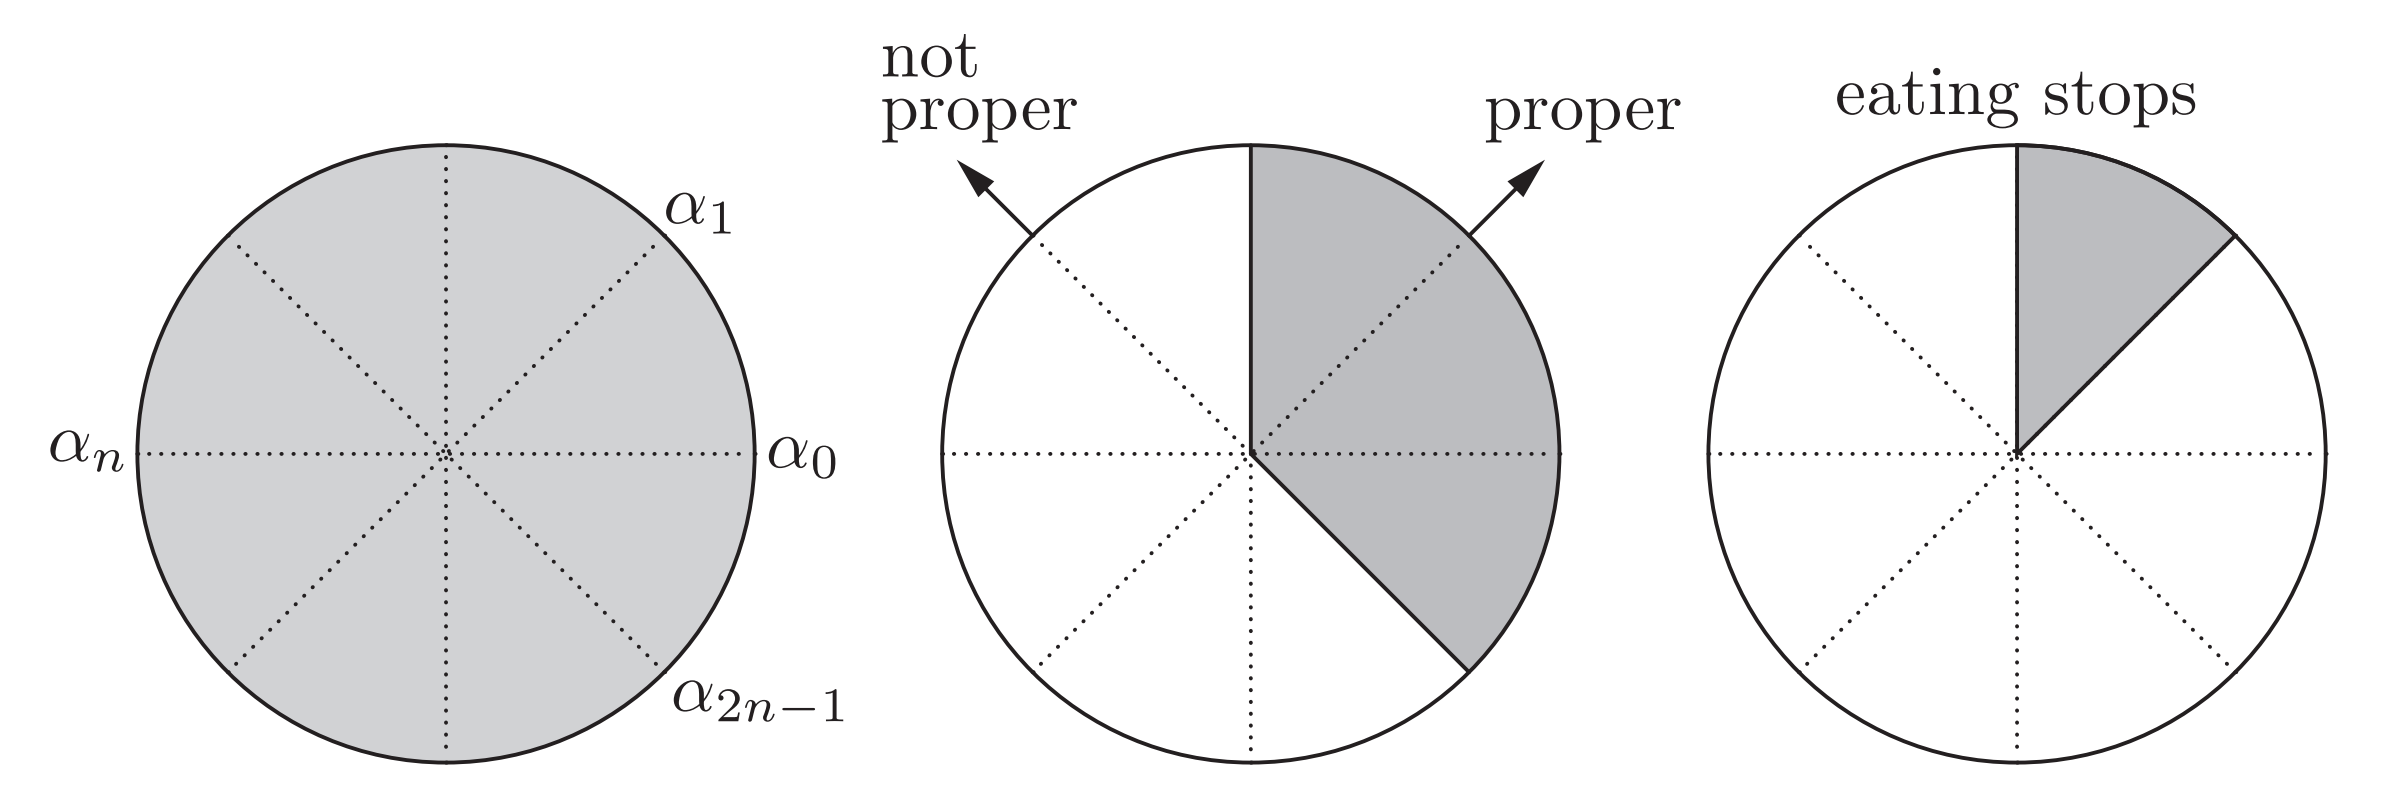
\includegraphics[width=1\linewidth]{p6.png}
\end{figure}

\begin{parts}
    \part[2] As a kickoff, let $v(i, j)$ be the tastiness of the $j$ slices counter-clockwise from angle $\alpha_i$. Write the formula over $v(i, j)$. 

    \begin{solution}
        \vspace{1in}
    \end{solution}

    \part[2] Define your subproblem for this question.

    \begin{solution}
        \vspace{1in}
    \end{solution}

    \bonuspart[4] Give your Bellman equation to solve the subproblems. (Proof of correctness is not required) 

    \begin{solution}
        \vspace{4in}
    \end{solution}

    \bonuspart[2] What is the answer to this question in terms of the subproblems?

    \begin{solution}
        \vspace{1in}
    \end{solution}

    \newpage

    \bonuspart[2] Give an explanation and time complexity analysis of this algorithm.
    \begin{solution}
        \vspace{8in}
    \end{solution}

    
\end{parts}